
\documentclass{article}
\usepackage[utf8]{inputenc}
\usepackage{graphicx}
\usepackage{geometry}
 \geometry{
	 a4paper,
	 total={170mm,257mm},
	 left=20mm,
 	top=20mm,
 }
 
\title{CSIR:Electronically Timing Athletes\\
The Inevitables
}

\author{  
            Peter Rayner\\
            Dawie Pritchard\\
            Drew Langley\\
            Hendrik Jan van der Merwe\\
            Lyle Nel\\
        }


\begin{document}

\maketitle

\includegraphics[width=20cm,height=11cm,keepaspectratio]{group.JPG}

\newpage

\tableofcontents

\newpage


\section{Introduction}
From preliminary research we have indentified numerous key issues that need to be addressed in order to realise the product. A good deal of this document is dedicated to proposed solutions to these key issues, most of which lies between the track outdoors and the server indoors. That being said, we have come up with some value added features that we think the athletes will enjoy, which will hopefully lead to faster adoption and usage of the new system. The document is layed out such that we discuss solutions on the front-end first, after which we will move to backend and hardware.

\subsection{Front-end}
Website which the athletes will make use of will be styled using the Twitter Bootstrap framework in order to accommodate different screen sizes, thereby supporting both mobile and desktop devices.

\subsection{Persistence}
We have decided to make use of PostgreSQL as a database. It is well supported, stable and scales relatively well with demand. This however is not set in stone and the team is very comfortable with changing the database if the need arises.

\subsection{Between the track and the server}
Drawing from how RFID tracking is done for large scale triathlons and similar events, we have identified a few key components. The bill of materials follows at the bottom of this section stipulating the costs of each compomenent. In the case that there are numerous options to consider, we show the best candidates while making recommendations for the most effective component for the job, both functional and cost wise.

\subsubsection{RFID tags}
Firstly we need to be able to attach an RFID tag to the athlete, the best solution we have found that is most convenient to attach and comfortable for the athlete to wear is the Triathlon UHF RFID Strap Tag, costing about \$1.1 per tag. It is extremely thin and light, so the athlete will not notice an uneven distribution of weight between feet. It is however a use once tag, which makes it expensive in the long run and requires that the unique ID of the tag be captured before each session. This is ideal for athletes that are not regulars at the track. For regular athletes, we recommend the HuTag XC1 UHF RFID Tag, it is somewhat heavier, weighing 24g, however, it is reusable and still quite cost effective at about \$7 per tag, droppping to \$3.24 per tag when ordered in bulk.

\subsubsection{RFID Antenna}
For the antenna, we recommend a mat which the athlete can run over to capture the time they pass the threshold. The Times-7 RFID Race Timing Antenna System seems like a good fit, it is 1.2m long which gives the athlete sufficient space to run over without distracting them. For events that do not stretch a perfect round trip of the track two of these mats will be needed, one for the start and one for the end.

\subsubsection{RFID Receiver}
The receiver gets attached to the mat antenna in order to read the RFID tag as it passes. We recommend the ThingMagic USB Plus+ RFID Reader for the following reasons. It has a host API that supports a good amount of languages while being relatively easy to communicate with. In addition it is powered and can be communicated with through usb, which we will see is important for the sections following. It is also the most cost effective and mobile unit we could find.


 


\subsection{Technologies}
\textbf{RFID Communication} \\
If a Raspberry Pi can be used:  
\begin{itemize}
	\item JEE
	\item JDBC
	\item JPA
	\item WildFly
Wildfly 10 will be the server that is used. The application will be coded in j2ee and then deployed on the wildfly server. The JDBC(java database connection) will be set up on wildfly itself using the wildfly API. JPA will be used for accessing, persisting and managing data between the java objects and the database. The wildfly server can be used in conjunction with  the raspberry pi to access the data. 
\end{itemize}
\textbf{Web Portal} 
\begin{itemize}
	\item HTML
	\item CSS / Bootstrap
	\item PHP
	\item JavaScript / JQuery / AJAX
\end{itemize}
\textbf{Database} \\
PostgreSQL

\subsection{Deployment Diagram} 
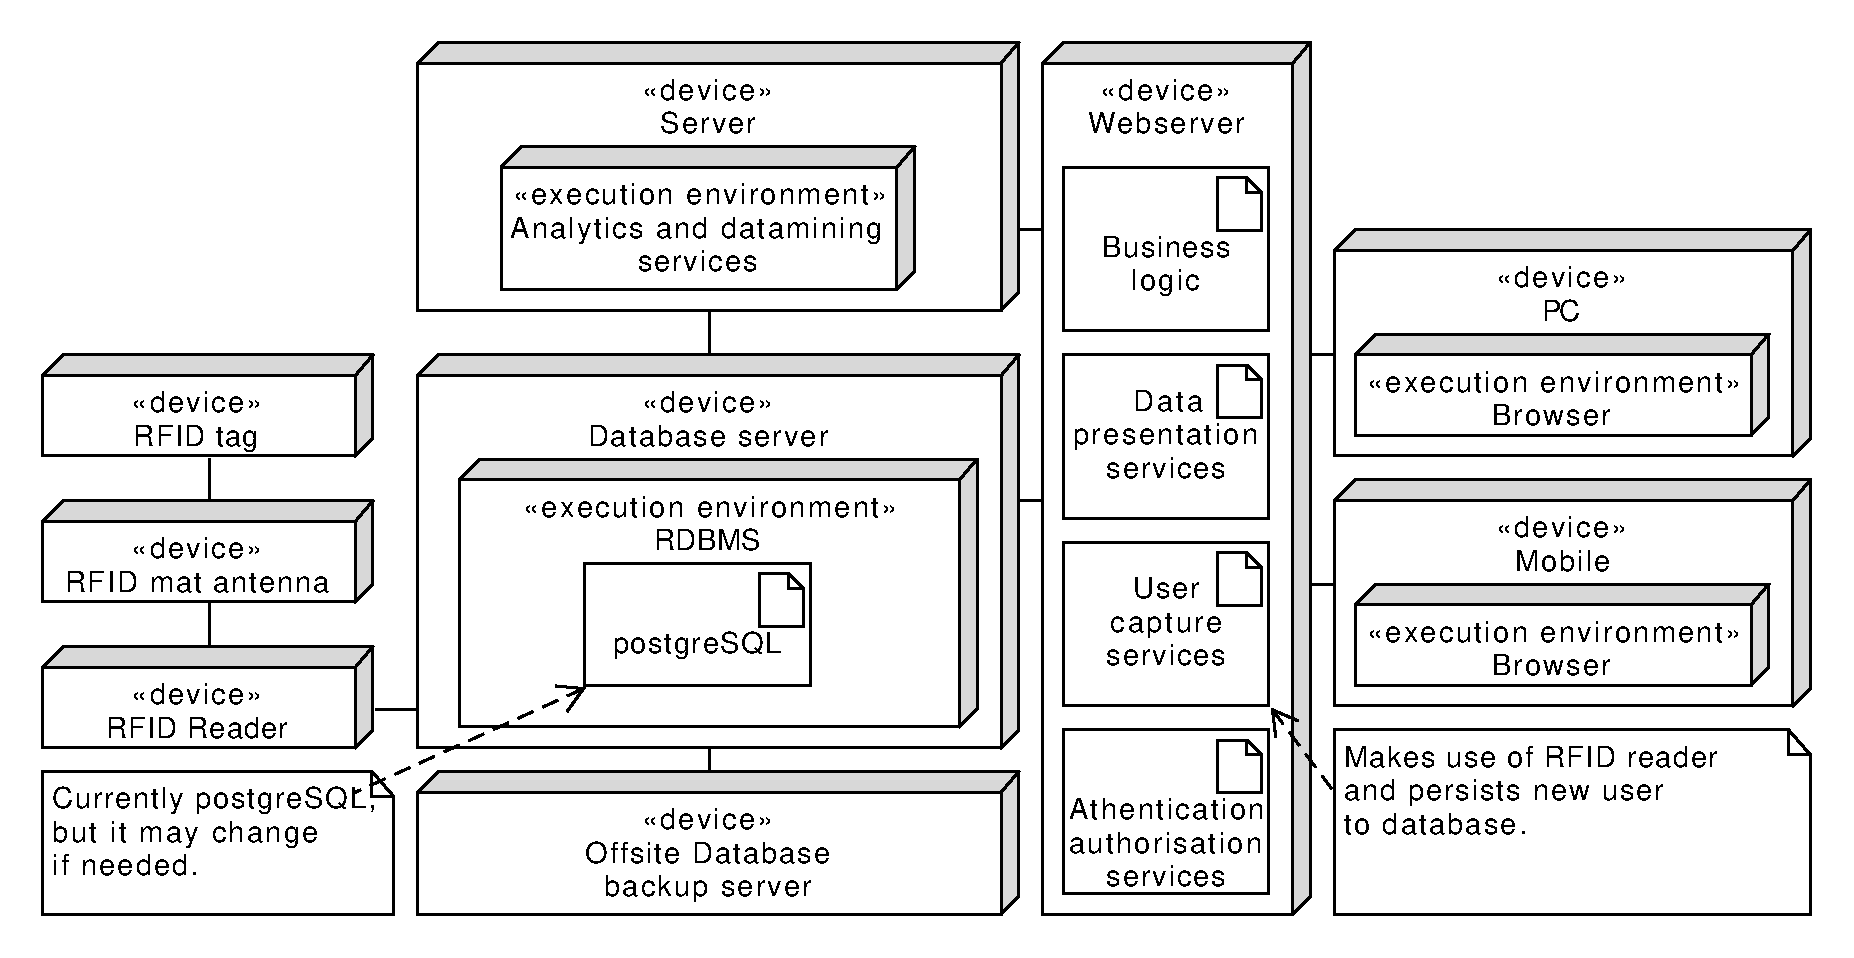
\includegraphics[width=18cm,height=11cm,keepaspectratio]{ETA-Deployment.pdf}

\section{Development Methodology}
We will be using the Agile Methodology. By making a backlog of work to be done and by completing deadlines in short iterations or sprints. We will meet daily by making use of  Slack Messaging Platform to discuss the progress as well as obstacles and how to overcome these obstacles by getting input from each member. We will also define when these deadlines are and make sure we keep to the schedule. We will meet everytime we are done with a deadline to reflect on the work done. \\ \\
At each deadline or meeting we will meet with the client to make sure that they are kept up to date with our progress. We will also meet with the client when there are concerns or obstacles to overcome to make sure the client aware about obstacles we are facing. The client will be kept up to date each week with the progress of the project.


\section{Team Details}
\subsection{Dawie Pritchard}
\textbf{Skills:}
\begin{itemize}
 	\item Human Computer Interaction
 	\item Trends, Visual Design 
 	\item Multimedia Specialist
 	\item Computer Scientist
\end {itemize}
\textbf{Technologies known:}
\begin{itemize}
	\item C
 	\item C++
 	\item C-Sharp
 	\item CSS
 	\item Bootstrap
 	\item Java
 	\item Python
 	\item Javascript / AngularJS / ExpressJS / NodeJS / JQUERY
 	\item MongoDB / NoSQL
 	\item Php
 	\item SQL
 	\item HTML5
 	\item XML
 \end{itemize}
\textbf{Stengths:} 
\begin{itemize}
	\item Front-End
	\item Back-End development
\end{itemize}

\newpage
\subsection {Peter Rayner}

\textbf{Front-end developer with knowledge of:}
\begin{itemize}
 	\item Artifical Intelligence
 	\item Data structures 
 	\item Website design 
 	\item Databases and human computer interaction(user experience)
 \end{itemize}
\textbf{Technologies known:}
\begin{itemize}
	\item C++ 
	\item C 
	\item C\# 
	\item Java 
	\item PHP
	\item mySQL
	\item postgreSQL
	\item JavaScript 
	\item Python 
	\item Assembly 
	\item AngularJS  
	\item Bootstrap
 \end{itemize}
\textbf{Previous industry experience:}\\
Working at Barclays CIB in big data and analytics.
\\
\newpage
\subsection {Hendrik Jan van der Merwe} 
\textbf{University level knowledge of:}
\begin{itemize}
 	\item Data structures
 	\item Databases
 	\item Human Computer Interaction focussing on User Experience
 	\item System Design
\end{itemize}
\textbf{Technologies known:}
\begin{itemize}
	\item C++
	\item C\#
	\item Java
	\item SQL / MySQL
	\item MongoDB
	\item PHP
	\item JavaScript / AJAX / JQuery / NodeJS / ExpressJS
	\item HTML / CSS / Bootstrap
	\item XML
\end{itemize}
\textbf{Strengths:}
\begin{itemize}
	\item Database Design
	\item Backend Development
\end{itemize}

\newpage
\subsection {Lyle Nel}
\textbf{Qualifications:} \\
I hold a BTEC in software engineering, which included project management as part of the curriculum.
I also hold a BSc in Computer Systems, with relevant subjects such as Software Engineering, Operations management, Knowledge management, Professional development, and Artificial intelligence.\\ \\
\textbf{Digital electronics:} \\
I have worked with Atmel and ARM microprocessors as well as on the arduino platform. In addition I am familiar with most of the common components of a digital circuit including 7400 series and 4000 series integrated circuits. \\ \\
\textbf{Computer Hardware:} \\
I am familiar with all standard consumer hardware and some server hardware. I maintain my own server cluster at home for running experiment. \\ \\
\textbf{Artificial intelligence} \\
I am most experienced in genetic algorithms and I am the author of an open source project that cracks passwords using genetic algorithms. The was one of the top 3 trending projects on github and hackernews a while back. See https://github.com/lyle-nel/siga. In general I am very comfortable with solving problems within the domain of AI. \\ \\
\textbf{Languages} \\
C, C++ including the new C++11, C++14 and C++17 ISO standards, Bash, Python, Javascript, Java, Lisp and Prolog. The language that I am most comfortable with is C++. When I conduct experiment on large datasets I use a mixture between C++, Python and Bash. \\ \\
\textbf{Platforms} \\
I do all of my work in a Linux environment.

\newpage
\subsection {Drew Langley}
Third year BIS Multimedia student with experience in UX and HCI, animation and 3D modelling, Web design and databases as well as proficiency in programming. I am currently studying networks, software engineering and Artificial Intelligence. \\ \\
\textbf{Technologies known:}
\begin{itemize}
	\item HTML
	\item CSS 
	\item JS / AngularJS / NodeJS / JQuery 
	\item PHP 
	\item SQL
	\item MongoDB
	\item Java 
	\item C++ 
	\item C 
	\item C\# 
	\item Python 
	\item Assembly
\end{itemize}
\textbf{Experience:} \\
Designed and developed www.ugandaprohunts.com

\textbf{Stengths:} 
\begin{itemize}
	\item Front-End
	\item Back-End development
\end{itemize}

\end{document}
